\documentclass[aspectratio=169]{beamer}
\usepackage{amsmath, amssymb}
\usepackage{graphicx}
\usepackage{xcolor}
\usepackage{tikz}
\usetikzlibrary{arrows.meta}
\usetikzlibrary{positioning}
\tikzset{
    sommet/.style = {circle, draw, on grid},
    >=Latex
}

% Metropolis theme
\usetheme{metropolis}
\usefonttheme[onlymath]{serif}
\metroset{progressbar=frametitle}
\metroset{titleformat=smallcaps}
\metroset{numbering=fraction}
\metroset{block=fill}
\definecolor{mypink}{HTML}{e91e63}
\setbeamercolor{alerted text}{fg=mypink}

\makeatletter
\setlength{\metropolis@titleseparator@linewidth}{1pt}
\setlength{\metropolis@progressonsectionpage@linewidth}{1.5pt}
\setlength{\metropolis@progressinheadfoot@linewidth}{2.5pt}
\makeatother

\title{Combinatorial Auctions with Restricted Complements}
\subtitle{An article by I. Abraham, M. Babaioff, S. Dughmi and T. Roughgarden}
\author{Hugo \textsc{Boulier}, Hugo \textsc{Francon} \& Igor \textsc{Martayan}}
\date{November 8, 2021}

\begin{document}

{\metroset{background=dark}\maketitle}

\begin{frame}{Introduction}
    \begin{columns}
        \column{0.6\textwidth}
        \begin{itemize}
            \item Auction with $n$ bidders and $m$ items
            \item Some item groups gain added value when purchased together
            \item Use of hyperedges to model these preferences
        \end{itemize}

        \column{0.4\textwidth}
        \begin{figure}[H]
            \begin{tikzpicture}[node distance=0.25cm and 0.25cm, font=\small]
                \node (complet) [inner sep=1pt] {10};
                \node (galette) [label={\scriptsize 0.5}, above left=of complet] {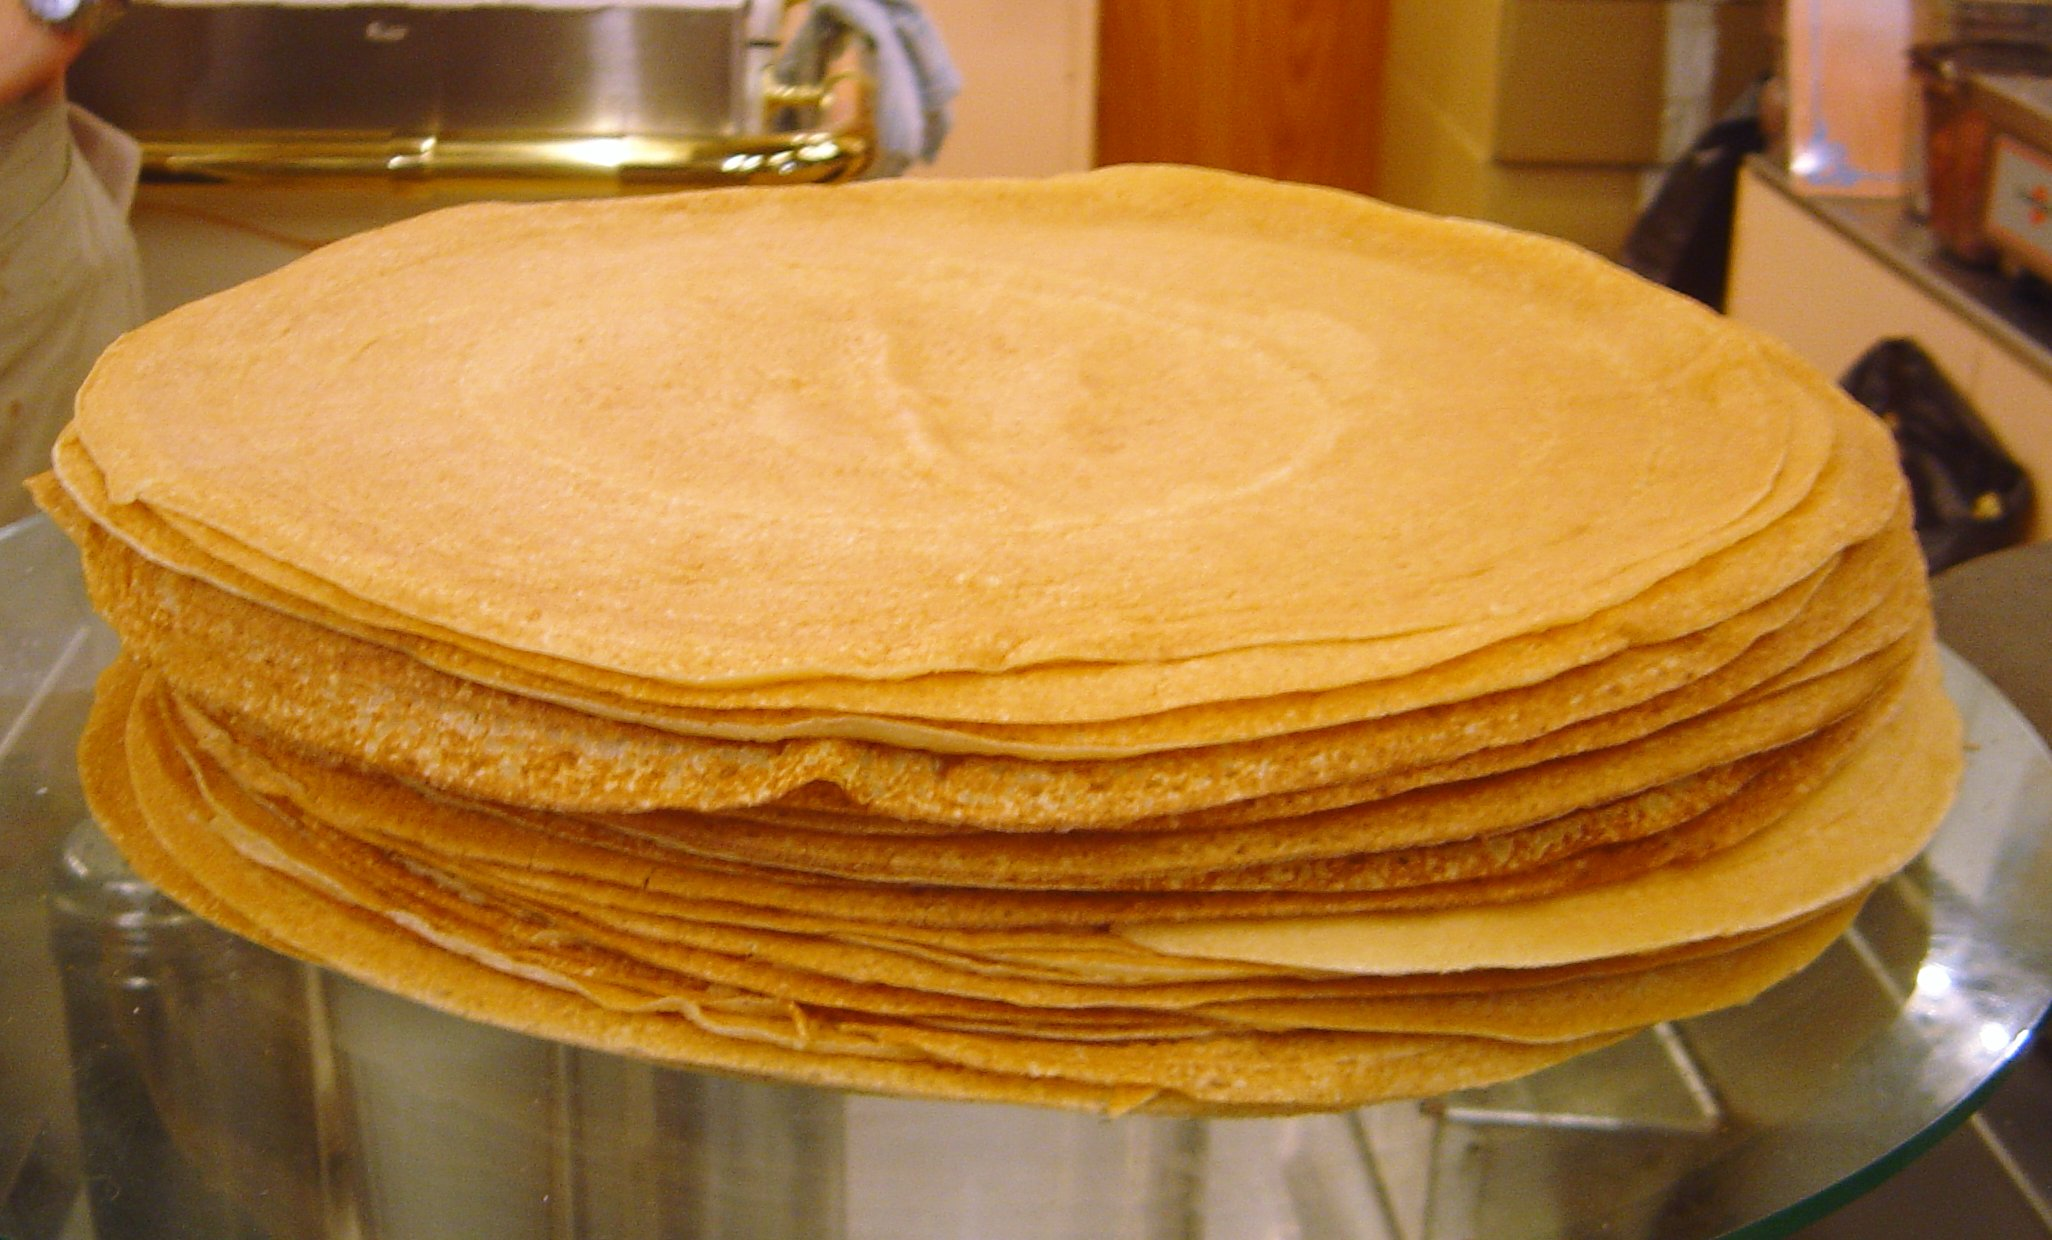
\includegraphics[width=0.4\textwidth]{img/crepe.jpg}};
                \node (oeuf) [label={\scriptsize 2.5}, above right=of complet] {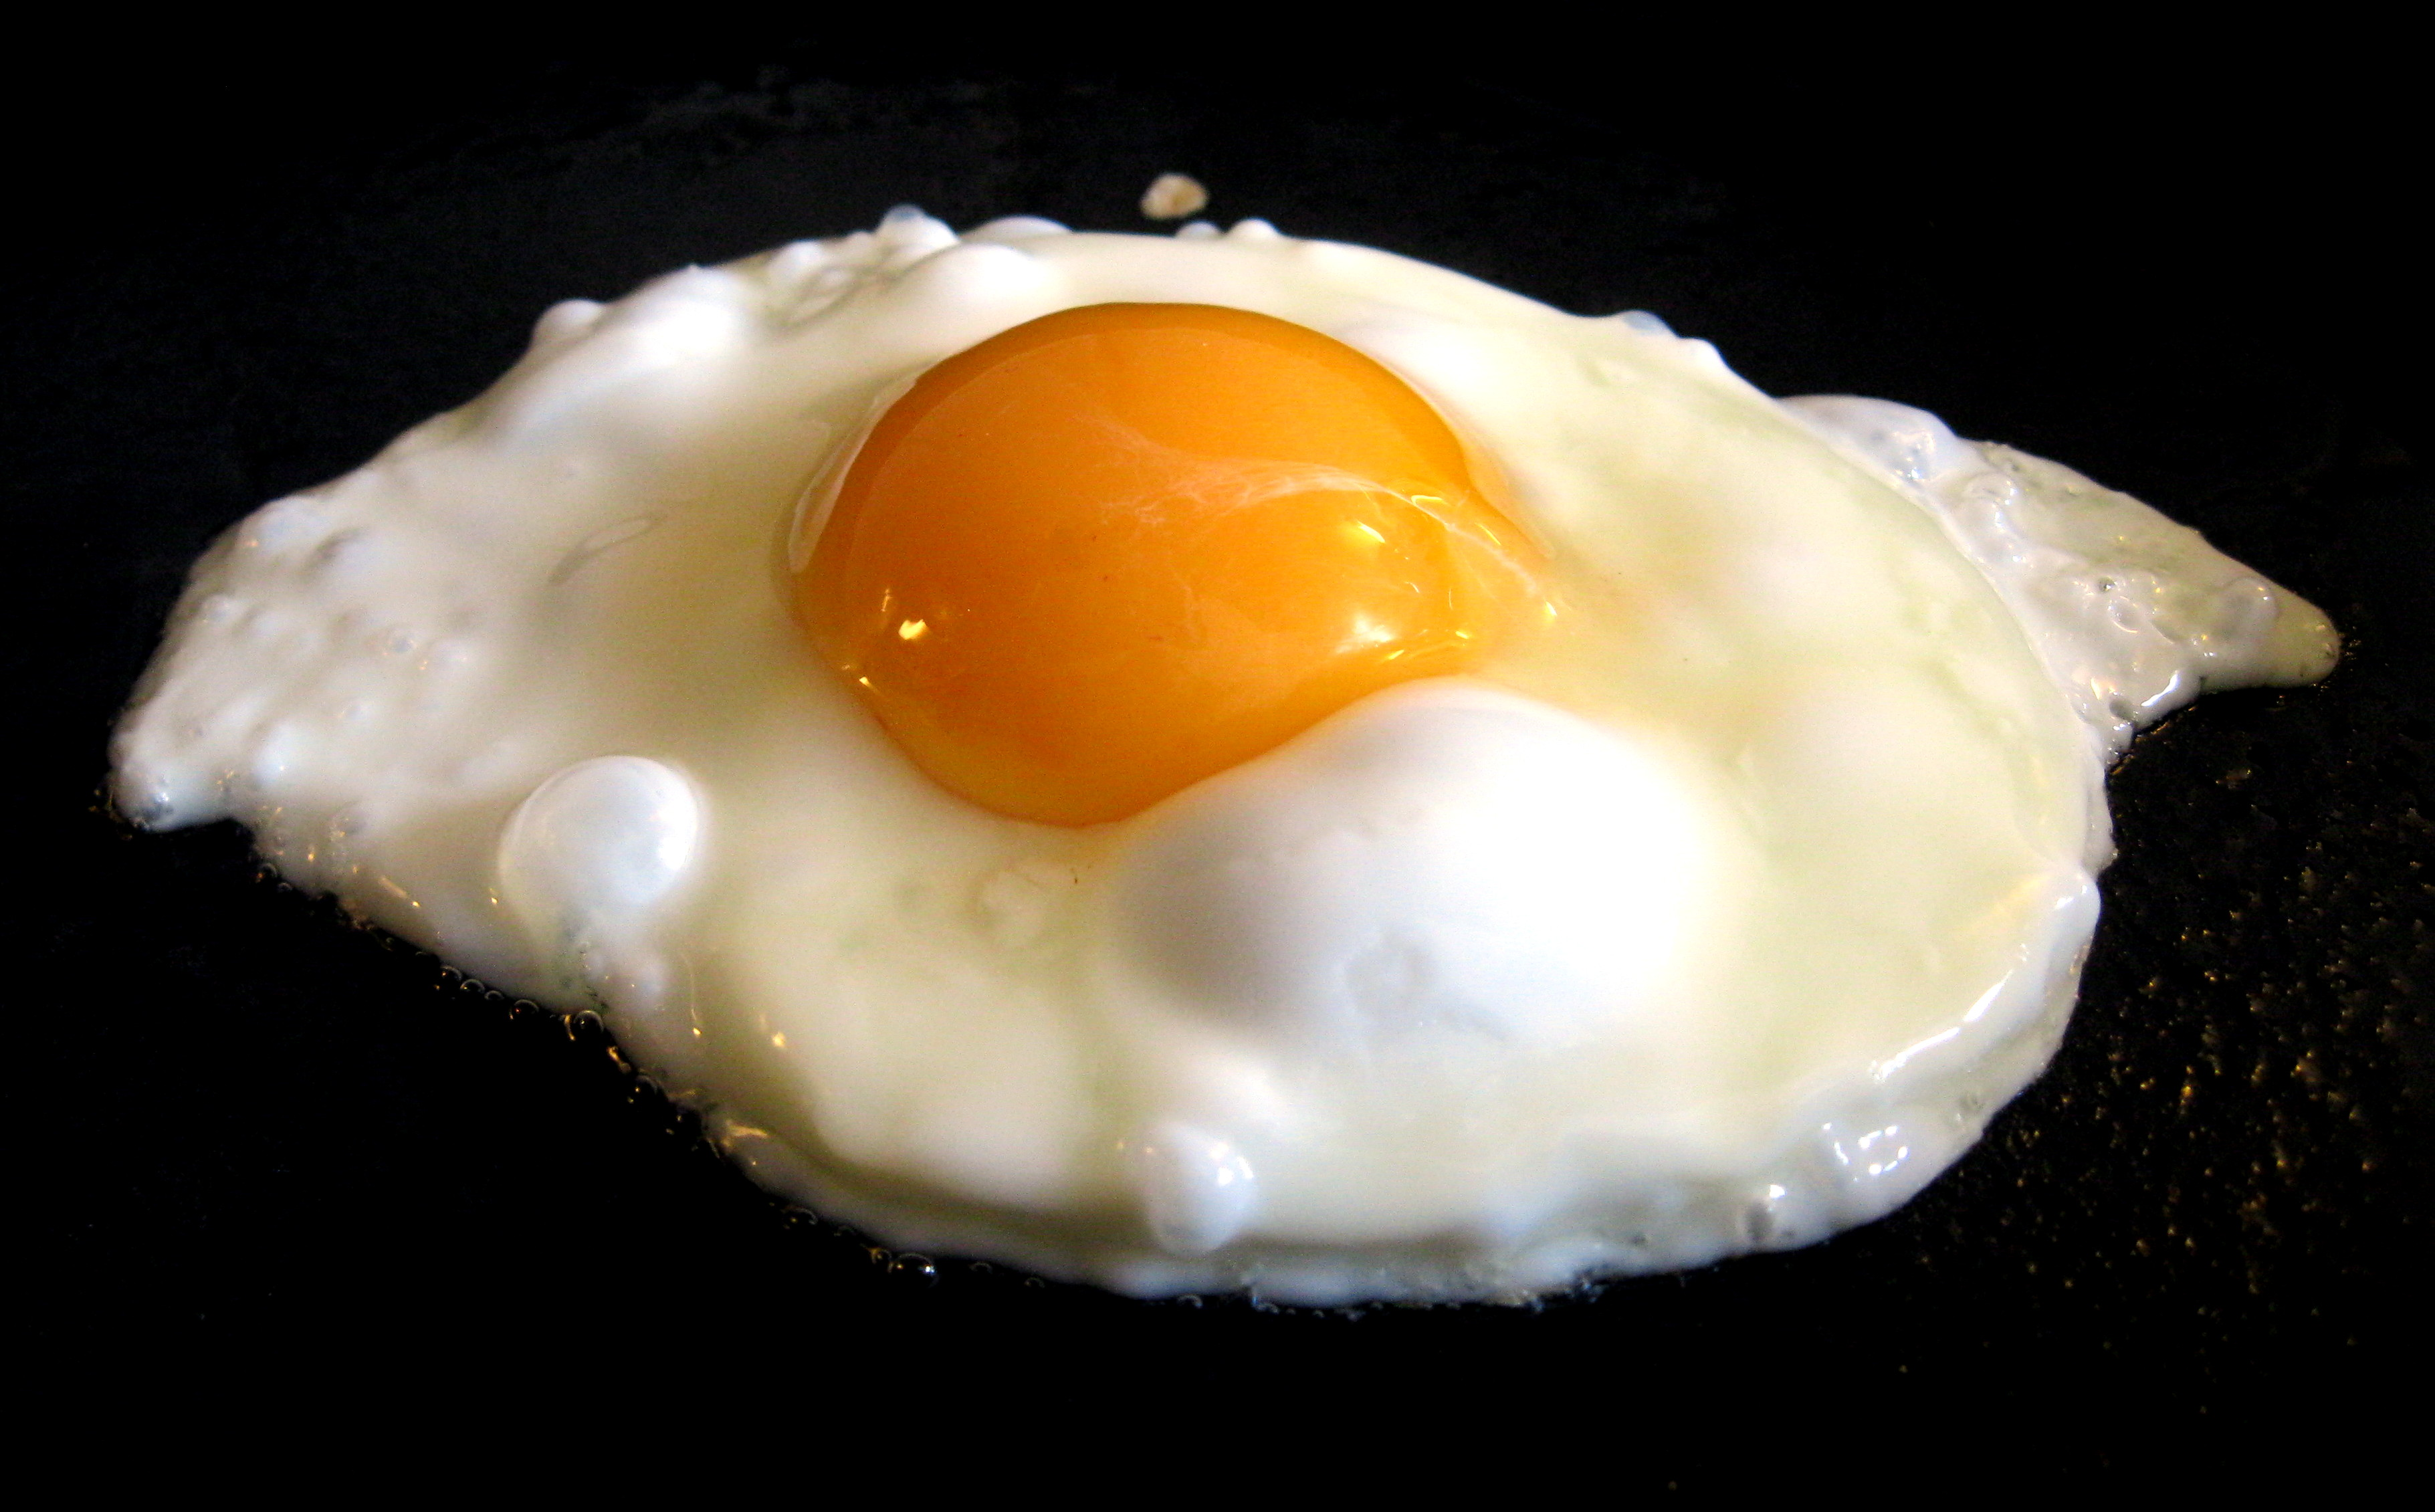
\includegraphics[width=0.4\textwidth]{img/oeuf.jpg}};
                \node (jambon) [label={\scriptsize 1.5}, below left=of complet] {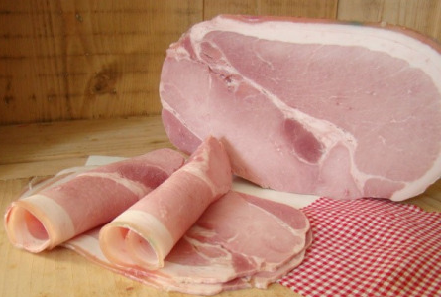
\includegraphics[width=0.4\textwidth]{img/jambon.png}};
                \node (fromage) [label={\scriptsize 2.5}, below right=of complet] {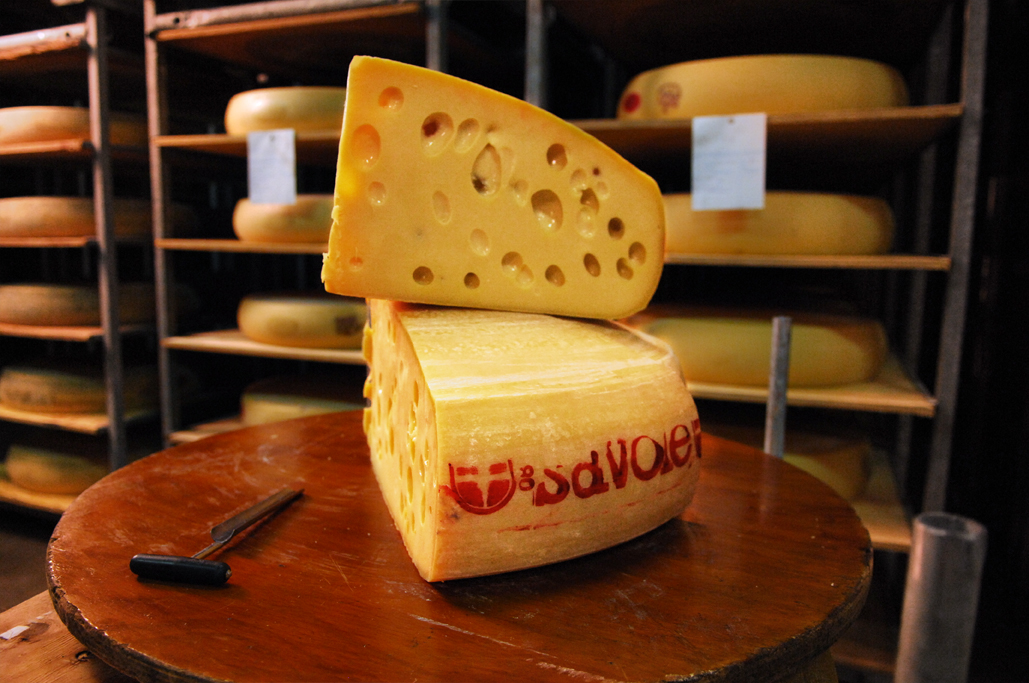
\includegraphics[width=0.4\textwidth]{img/fromage.jpg}};
                \draw (galette) -- (complet) -- (jambon) -- (complet) -- (oeuf) -- (complet) -- (fromage);
            \end{tikzpicture}
        \end{figure}
    \end{columns}
\end{frame}

\begin{frame}{Core Questions}
    \begin{enumerate}
        \item Polynomial-time approximation for \alert{planar graphs}?
        \item Polynomial-time approximation for \alert{hypergraphs}?
        \item \alert{Truthful version} of this approximation?
    \end{enumerate}
\end{frame}

{\metroset{background=dark}\section{Polynomial-time approximation for planar graphs}}

\begin{frame}{Polynomial-time approximation maximizing welfare}
    \begin{columns}
        \column{0.6\textwidth}
        G is a planar graph

        \begin{block}{theorem}
            For any $\varepsilon > 0$, we can compute a $(1 + \varepsilon)$-approximation of the optimal welfare repartition in polynomial-time.
        \end{block}

        \begin{block}{theorem}
            Once combined with VCG auctions, this mechanism is truthful.
        \end{block}

        \column{0.4\textwidth}
        On se restreint aux graphe auquel on a enlevé des neouds à une certaine distance (variable) de la racine

        Pour chacun de ces graphes, on calcule les allocations, et pour l'un d'entre eux on a une (1+varepsilon)-approximation


    \end{columns}
\end{frame}

\begin{frame}[standout]
    Can we generalize this approach ?
\end{frame}

\begin{frame}{Approximate welfare maximization algorithm}
    \begin{columns}
        \column{0.6\textwidth}
        We generalize to $r$-hypergraph

        \begin{block}{theorem}
            ...
        \end{block}

        Unfortunately, this mechanism is not truthful.

        \column{0.4\textwidth}
        ...
    \end{columns}
\end{frame}

\begin{frame}[standout]
    Can we solve this problem ?
\end{frame}

\begin{frame}{A truthful approximation mechanism}
    \begin{columns}
        \column{0.6\textwidth}
        ...

        \column{0.4\textwidth}
        ...
    \end{columns}
\end{frame}

\begin{frame}{Conclusion}
    ...
\end{frame}

\end{document}
